% Created by tikzDevice version 0.12.3 on 2020-05-15 17:19:15
% !TEX encoding = UTF-8 Unicode
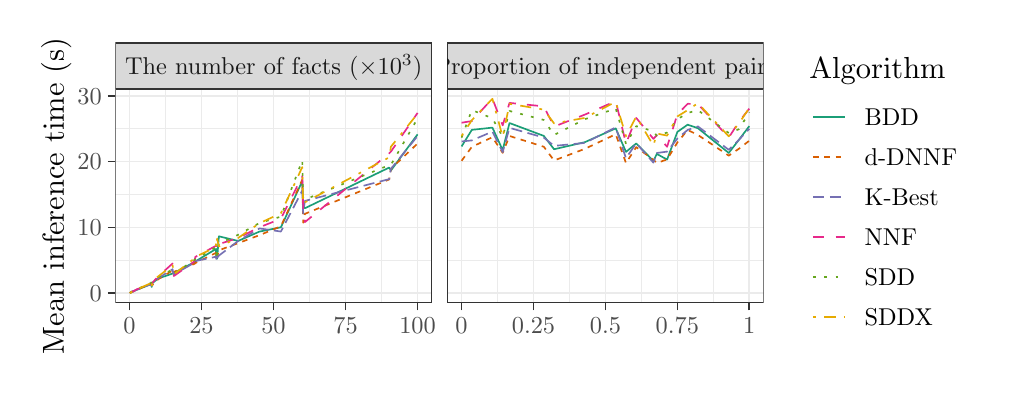
\begin{tikzpicture}[x=1pt,y=1pt]
\definecolor{fillColor}{RGB}{255,255,255}
\path[use as bounding box,fill=fillColor,fill opacity=0.00] (0,0) rectangle (346.90,130.09);
\begin{scope}
\path[clip] (  0.00,  0.00) rectangle (346.90,130.09);
\definecolor{drawColor}{RGB}{255,255,255}
\definecolor{fillColor}{RGB}{255,255,255}

\path[draw=drawColor,line width= 0.6pt,line join=round,line cap=round,fill=fillColor] (  0.00,  0.00) rectangle (346.90,130.09);
\end{scope}
\begin{scope}
\path[clip] ( 31.71, 30.69) rectangle (146.09,108.01);
\definecolor{fillColor}{RGB}{255,255,255}

\path[fill=fillColor] ( 31.71, 30.69) rectangle (146.09,108.01);
\definecolor{drawColor}{gray}{0.92}

\path[draw=drawColor,line width= 0.3pt,line join=round] ( 31.71, 46.03) --
	(146.09, 46.03);

\path[draw=drawColor,line width= 0.3pt,line join=round] ( 31.71, 69.81) --
	(146.09, 69.81);

\path[draw=drawColor,line width= 0.3pt,line join=round] ( 31.71, 93.59) --
	(146.09, 93.59);

\path[draw=drawColor,line width= 0.3pt,line join=round] ( 49.77, 30.69) --
	( 49.77,108.01);

\path[draw=drawColor,line width= 0.3pt,line join=round] ( 75.80, 30.69) --
	( 75.80,108.01);

\path[draw=drawColor,line width= 0.3pt,line join=round] (101.84, 30.69) --
	(101.84,108.01);

\path[draw=drawColor,line width= 0.3pt,line join=round] (127.87, 30.69) --
	(127.87,108.01);

\path[draw=drawColor,line width= 0.6pt,line join=round] ( 31.71, 34.14) --
	(146.09, 34.14);

\path[draw=drawColor,line width= 0.6pt,line join=round] ( 31.71, 57.92) --
	(146.09, 57.92);

\path[draw=drawColor,line width= 0.6pt,line join=round] ( 31.71, 81.70) --
	(146.09, 81.70);

\path[draw=drawColor,line width= 0.6pt,line join=round] ( 31.71,105.48) --
	(146.09,105.48);

\path[draw=drawColor,line width= 0.6pt,line join=round] ( 36.75, 30.69) --
	( 36.75,108.01);

\path[draw=drawColor,line width= 0.6pt,line join=round] ( 62.79, 30.69) --
	( 62.79,108.01);

\path[draw=drawColor,line width= 0.6pt,line join=round] ( 88.82, 30.69) --
	( 88.82,108.01);

\path[draw=drawColor,line width= 0.6pt,line join=round] (114.85, 30.69) --
	(114.85,108.01);

\path[draw=drawColor,line width= 0.6pt,line join=round] (140.89, 30.69) --
	(140.89,108.01);
\definecolor{drawColor}{RGB}{27,158,119}

\path[draw=drawColor,line width= 0.6pt,line join=round] ( 36.91, 34.22) --
	( 37.07, 34.28) --
	( 37.38, 34.45) --
	( 37.80, 34.74) --
	( 38.00, 34.74) --
	( 39.25, 35.27) --
	( 44.64, 37.45) --
	( 44.80, 36.38) --
	( 45.11, 37.84) --
	( 47.17, 39.46) --
	( 52.37, 41.24) --
	( 52.53, 41.31) --
	( 52.84, 41.51) --
	( 60.26, 45.33) --
	( 60.58, 45.62) --
	( 67.99, 50.08) --
	( 68.15, 47.64) --
	( 68.31, 50.15) --
	( 68.46, 46.59) --
	( 69.09, 54.70) --
	( 76.04, 53.02) --
	( 83.77, 56.41) --
	( 91.50, 57.95) --
	( 99.23, 74.63) --
	( 99.55, 65.78) --
	(100.17, 64.84) --
	(130.63, 79.54) --
	(131.26, 78.48) --
	(140.89, 91.54);
\definecolor{drawColor}{RGB}{217,95,2}

\path[draw=drawColor,line width= 0.6pt,dash pattern=on 2pt off 2pt ,line join=round] ( 36.91, 34.20) --
	( 37.07, 34.26) --
	( 37.38, 34.41) --
	( 37.80, 34.70) --
	( 38.00, 34.68) --
	( 39.25, 35.23) --
	( 44.64, 37.74) --
	( 44.80, 37.05) --
	( 45.11, 37.14) --
	( 47.17, 39.19) --
	( 52.37, 42.35) --
	( 52.53, 40.98) --
	( 52.84, 41.86) --
	( 60.26, 44.75) --
	( 60.58, 45.01) --
	( 67.99, 48.70) --
	( 68.15, 46.51) --
	( 68.31, 47.05) --
	( 68.46, 47.32) --
	( 69.09, 49.64) --
	( 76.04, 52.22) --
	( 83.77, 55.11) --
	( 91.50, 58.33) --
	( 99.23, 75.16) --
	( 99.55, 59.59) --
	(100.17, 62.82) --
	(130.63, 75.24) --
	(131.26, 79.11) --
	(140.89, 88.23);
\definecolor{drawColor}{RGB}{117,112,179}

\path[draw=drawColor,line width= 0.6pt,dash pattern=on 4pt off 2pt ,line join=round] ( 36.91, 34.22) --
	( 37.07, 34.33) --
	( 37.38, 34.49) --
	( 37.80, 34.77) --
	( 38.00, 34.77) --
	( 39.25, 35.37) --
	( 44.64, 37.40) --
	( 44.80, 36.84) --
	( 45.11, 37.68) --
	( 47.17, 39.58) --
	( 52.37, 42.81) --
	( 52.53, 41.77) --
	( 52.84, 40.98) --
	( 60.26, 45.16) --
	( 60.58, 45.74) --
	( 67.99, 47.31) --
	( 68.15, 46.52) --
	( 68.31, 48.59) --
	( 68.46, 46.96) --
	( 69.09, 47.72) --
	( 76.04, 52.99) --
	( 83.77, 57.55) --
	( 91.50, 56.42) --
	( 99.23, 71.23) --
	( 99.55, 62.93) --
	(100.17, 67.49) --
	(130.63, 75.36) --
	(131.26, 79.09) --
	(140.89, 90.92);
\definecolor{drawColor}{RGB}{231,41,138}

\path[draw=drawColor,line width= 0.6pt,dash pattern=on 4pt off 4pt ,line join=round] ( 36.91, 34.22) --
	( 37.07, 34.29) --
	( 37.38, 34.48) --
	( 37.80, 34.79) --
	( 38.00, 34.74) --
	( 39.25, 35.45) --
	( 44.64, 37.64) --
	( 44.80, 37.18) --
	( 45.11, 37.98) --
	( 47.17, 40.20) --
	( 52.37, 44.88) --
	( 52.53, 42.06) --
	( 52.84, 40.35) --
	( 60.26, 45.65) --
	( 60.58, 47.25) --
	( 67.99, 51.25) --
	( 68.15, 51.16) --
	( 68.31, 51.25) --
	( 68.46, 52.79) --
	( 69.09, 51.87) --
	( 76.04, 54.08) --
	( 83.77, 57.97) --
	( 91.50, 61.03) --
	( 99.23, 76.47) --
	( 99.55, 65.20) --
	(100.17, 59.83) --
	(130.63, 84.66) --
	(131.26, 85.31) --
	(140.89, 99.29);
\definecolor{drawColor}{RGB}{102,166,30}

\path[draw=drawColor,line width= 0.6pt,dash pattern=on 1pt off 3pt ,line join=round] ( 36.91, 34.24) --
	( 37.07, 34.31) --
	( 37.38, 34.48) --
	( 37.80, 34.81) --
	( 38.00, 34.77) --
	( 39.25, 35.45) --
	( 44.64, 37.88) --
	( 44.80, 38.54) --
	( 45.11, 38.69) --
	( 47.17, 39.95) --
	( 52.37, 42.70) --
	( 52.53, 41.93) --
	( 52.84, 41.20) --
	( 60.26, 46.14) --
	( 60.58, 46.43) --
	( 67.99, 50.70) --
	( 68.15, 47.87) --
	( 68.31, 50.28) --
	( 68.46, 47.98) --
	( 69.09, 52.07) --
	( 76.04, 55.24) --
	( 83.77, 59.51) --
	( 91.50, 61.81) --
	( 99.23, 82.15) --
	( 99.55, 68.77) --
	(100.17, 67.98) --
	(130.63, 80.43) --
	(131.26, 80.51) --
	(140.89, 97.30);
\definecolor{drawColor}{RGB}{230,171,2}

\path[draw=drawColor,line width= 0.6pt,dash pattern=on 1pt off 3pt on 4pt off 3pt ,line join=round] ( 36.91, 34.20) --
	( 37.07, 34.32) --
	( 37.38, 34.47) --
	( 37.80, 34.80) --
	( 38.00, 34.78) --
	( 39.25, 35.44) --
	( 44.64, 37.83) --
	( 44.80, 36.07) --
	( 45.11, 38.73) --
	( 47.17, 40.20) --
	( 52.37, 44.23) --
	( 52.53, 43.29) --
	( 52.84, 40.97) --
	( 60.26, 46.70) --
	( 60.58, 47.28) --
	( 67.99, 50.76) --
	( 68.15, 52.81) --
	( 68.31, 51.86) --
	( 68.46, 53.84) --
	( 69.09, 51.03) --
	( 76.04, 54.08) --
	( 83.77, 59.44) --
	( 91.50, 63.01) --
	( 99.23, 79.72) --
	( 99.55, 66.18) --
	(100.17, 66.97) --
	(130.63, 83.22) --
	(131.26, 87.08) --
	(140.89, 98.99);
\definecolor{drawColor}{gray}{0.20}

\path[draw=drawColor,line width= 0.6pt,line join=round,line cap=round] ( 31.71, 30.69) rectangle (146.09,108.01);
\end{scope}
\begin{scope}
\path[clip] (151.59, 30.69) rectangle (265.96,108.01);
\definecolor{fillColor}{RGB}{255,255,255}

\path[fill=fillColor] (151.59, 30.69) rectangle (265.96,108.01);
\definecolor{drawColor}{gray}{0.92}

\path[draw=drawColor,line width= 0.3pt,line join=round] (151.59, 46.03) --
	(265.96, 46.03);

\path[draw=drawColor,line width= 0.3pt,line join=round] (151.59, 69.81) --
	(265.96, 69.81);

\path[draw=drawColor,line width= 0.3pt,line join=round] (151.59, 93.59) --
	(265.96, 93.59);

\path[draw=drawColor,line width= 0.3pt,line join=round] (169.78, 30.69) --
	(169.78,108.01);

\path[draw=drawColor,line width= 0.3pt,line join=round] (195.78, 30.69) --
	(195.78,108.01);

\path[draw=drawColor,line width= 0.3pt,line join=round] (221.77, 30.69) --
	(221.77,108.01);

\path[draw=drawColor,line width= 0.3pt,line join=round] (247.77, 30.69) --
	(247.77,108.01);

\path[draw=drawColor,line width= 0.6pt,line join=round] (151.59, 34.14) --
	(265.96, 34.14);

\path[draw=drawColor,line width= 0.6pt,line join=round] (151.59, 57.92) --
	(265.96, 57.92);

\path[draw=drawColor,line width= 0.6pt,line join=round] (151.59, 81.70) --
	(265.96, 81.70);

\path[draw=drawColor,line width= 0.6pt,line join=round] (151.59,105.48) --
	(265.96,105.48);

\path[draw=drawColor,line width= 0.6pt,line join=round] (156.79, 30.69) --
	(156.79,108.01);

\path[draw=drawColor,line width= 0.6pt,line join=round] (182.78, 30.69) --
	(182.78,108.01);

\path[draw=drawColor,line width= 0.6pt,line join=round] (208.77, 30.69) --
	(208.77,108.01);

\path[draw=drawColor,line width= 0.6pt,line join=round] (234.77, 30.69) --
	(234.77,108.01);

\path[draw=drawColor,line width= 0.6pt,line join=round] (260.76, 30.69) --
	(260.76,108.01);
\definecolor{drawColor}{RGB}{27,158,119}

\path[draw=drawColor,line width= 0.6pt,line join=round] (156.79, 87.17) --
	(160.50, 93.17) --
	(167.93, 93.97) --
	(171.64, 85.86) --
	(174.11, 95.63) --
	(186.49, 90.99) --
	(190.21, 86.16) --
	(201.35, 88.72) --
	(212.49, 93.71) --
	(216.20, 85.21) --
	(219.91, 88.26) --
	(226.10, 81.94) --
	(227.34, 84.46) --
	(231.05, 82.43) --
	(234.77, 92.42) --
	(238.48, 95.04) --
	(242.19, 93.76) --
	(253.34, 84.82) --
	(257.05, 89.64) --
	(260.76, 94.51);
\definecolor{drawColor}{RGB}{217,95,2}

\path[draw=drawColor,line width= 0.6pt,dash pattern=on 2pt off 2pt ,line join=round] (156.79, 81.98) --
	(160.50, 87.03) --
	(167.93, 90.51) --
	(171.64, 84.86) --
	(174.11, 90.95) --
	(186.49, 87.07) --
	(190.21, 82.10) --
	(201.35, 86.31) --
	(212.49, 91.58) --
	(216.20, 81.17) --
	(219.91, 86.92) --
	(226.10, 82.36) --
	(227.34, 81.20) --
	(231.05, 82.46) --
	(234.77, 88.61) --
	(238.48, 93.14) --
	(242.19, 91.31) --
	(253.34, 83.85) --
	(257.05, 86.37) --
	(260.76, 89.25);
\definecolor{drawColor}{RGB}{117,112,179}

\path[draw=drawColor,line width= 0.6pt,dash pattern=on 4pt off 2pt ,line join=round] (156.79, 88.97) --
	(160.50, 89.35) --
	(167.93, 92.54) --
	(171.64, 85.10) --
	(174.11, 93.89) --
	(186.49, 90.38) --
	(190.21, 87.37) --
	(201.35, 88.45) --
	(212.49, 94.07) --
	(216.20, 82.90) --
	(219.91, 88.35) --
	(226.10, 81.32) --
	(227.34, 84.81) --
	(231.05, 85.30) --
	(234.77, 90.02) --
	(238.48, 93.14) --
	(242.19, 94.41) --
	(253.34, 85.94) --
	(257.05, 89.62) --
	(260.76, 93.56);
\definecolor{drawColor}{RGB}{231,41,138}

\path[draw=drawColor,line width= 0.6pt,dash pattern=on 4pt off 4pt ,line join=round] (156.79, 95.74) --
	(160.50, 96.35) --
	(167.93,104.50) --
	(171.64, 94.79) --
	(174.11,102.91) --
	(186.49,101.65) --
	(190.21, 94.35) --
	(201.35, 98.68) --
	(212.49,103.55) --
	(216.20, 88.20) --
	(219.91, 97.47) --
	(226.10, 89.92) --
	(227.34, 91.22) --
	(231.05, 87.06) --
	(234.77, 98.75) --
	(238.48,102.58) --
	(242.19,102.50) --
	(253.34, 90.37) --
	(257.05, 96.15) --
	(260.76,100.82);
\definecolor{drawColor}{RGB}{102,166,30}

\path[draw=drawColor,line width= 0.6pt,dash pattern=on 1pt off 3pt ,line join=round] (156.79, 90.34) --
	(160.50,100.33) --
	(167.93, 97.34) --
	(171.64, 90.63) --
	(174.11, 99.99) --
	(186.49, 96.75) --
	(190.21, 91.32) --
	(201.35, 97.00) --
	(212.49,100.90) --
	(216.20, 88.11) --
	(219.91, 94.51) --
	(226.10, 92.66) --
	(227.34, 90.99) --
	(231.05, 92.19) --
	(234.77, 96.98) --
	(238.48, 99.26) --
	(242.19,100.29) --
	(253.34, 92.01) --
	(257.05, 93.41) --
	(260.76, 99.52);
\definecolor{drawColor}{RGB}{230,171,2}

\path[draw=drawColor,line width= 0.6pt,dash pattern=on 1pt off 3pt on 4pt off 3pt ,line join=round] (156.79, 90.96) --
	(160.50, 96.67) --
	(167.93,104.39) --
	(171.64, 90.59) --
	(174.11,102.58) --
	(186.49,100.48) --
	(190.21, 95.50) --
	(201.35, 97.48) --
	(212.49,103.31) --
	(216.20, 90.87) --
	(219.91, 97.96) --
	(226.10, 87.48) --
	(227.34, 91.85) --
	(231.05, 91.08) --
	(234.77, 98.02) --
	(238.48,100.29) --
	(242.19,102.81) --
	(253.34, 90.81) --
	(257.05, 95.58) --
	(260.76,101.07);
\definecolor{drawColor}{gray}{0.20}

\path[draw=drawColor,line width= 0.6pt,line join=round,line cap=round] (151.59, 30.69) rectangle (265.96,108.01);
\end{scope}
\begin{scope}
\path[clip] ( 31.71,108.01) rectangle (146.09,124.59);
\definecolor{drawColor}{gray}{0.20}
\definecolor{fillColor}{gray}{0.85}

\path[draw=drawColor,line width= 0.6pt,line join=round,line cap=round,fill=fillColor] ( 31.71,108.01) rectangle (146.09,124.59);
\definecolor{drawColor}{gray}{0.10}

\node[text=drawColor,anchor=base,inner sep=0pt, outer sep=0pt, scale=  0.88] at ( 88.90,113.27) {The number of facts ($\times 10^3$)};
\end{scope}
\begin{scope}
\path[clip] (151.59,108.01) rectangle (265.96,124.59);
\definecolor{drawColor}{gray}{0.20}
\definecolor{fillColor}{gray}{0.85}

\path[draw=drawColor,line width= 0.6pt,line join=round,line cap=round,fill=fillColor] (151.59,108.01) rectangle (265.96,124.59);
\definecolor{drawColor}{gray}{0.10}

\node[text=drawColor,anchor=base,inner sep=0pt, outer sep=0pt, scale=  0.88] at (208.77,113.27) {Proportion of independent pairs};
\end{scope}
\begin{scope}
\path[clip] (  0.00,  0.00) rectangle (346.90,130.09);
\definecolor{drawColor}{gray}{0.20}

\path[draw=drawColor,line width= 0.6pt,line join=round] ( 36.75, 27.94) --
	( 36.75, 30.69);

\path[draw=drawColor,line width= 0.6pt,line join=round] ( 62.79, 27.94) --
	( 62.79, 30.69);

\path[draw=drawColor,line width= 0.6pt,line join=round] ( 88.82, 27.94) --
	( 88.82, 30.69);

\path[draw=drawColor,line width= 0.6pt,line join=round] (114.85, 27.94) --
	(114.85, 30.69);

\path[draw=drawColor,line width= 0.6pt,line join=round] (140.89, 27.94) --
	(140.89, 30.69);
\end{scope}
\begin{scope}
\path[clip] (  0.00,  0.00) rectangle (346.90,130.09);
\definecolor{drawColor}{gray}{0.30}

\node[text=drawColor,anchor=base,inner sep=0pt, outer sep=0pt, scale=  0.88] at ( 36.75, 19.68) {0};

\node[text=drawColor,anchor=base,inner sep=0pt, outer sep=0pt, scale=  0.88] at ( 62.79, 19.68) {25};

\node[text=drawColor,anchor=base,inner sep=0pt, outer sep=0pt, scale=  0.88] at ( 88.82, 19.68) {50};

\node[text=drawColor,anchor=base,inner sep=0pt, outer sep=0pt, scale=  0.88] at (114.85, 19.68) {75};

\node[text=drawColor,anchor=base,inner sep=0pt, outer sep=0pt, scale=  0.88] at (140.89, 19.68) {100};
\end{scope}
\begin{scope}
\path[clip] (  0.00,  0.00) rectangle (346.90,130.09);
\definecolor{drawColor}{gray}{0.20}

\path[draw=drawColor,line width= 0.6pt,line join=round] (156.79, 27.94) --
	(156.79, 30.69);

\path[draw=drawColor,line width= 0.6pt,line join=round] (182.78, 27.94) --
	(182.78, 30.69);

\path[draw=drawColor,line width= 0.6pt,line join=round] (208.77, 27.94) --
	(208.77, 30.69);

\path[draw=drawColor,line width= 0.6pt,line join=round] (234.77, 27.94) --
	(234.77, 30.69);

\path[draw=drawColor,line width= 0.6pt,line join=round] (260.76, 27.94) --
	(260.76, 30.69);
\end{scope}
\begin{scope}
\path[clip] (  0.00,  0.00) rectangle (346.90,130.09);
\definecolor{drawColor}{gray}{0.30}

\node[text=drawColor,anchor=base,inner sep=0pt, outer sep=0pt, scale=  0.88] at (156.79, 19.68) {0};

\node[text=drawColor,anchor=base,inner sep=0pt, outer sep=0pt, scale=  0.88] at (182.78, 19.68) {0.25};

\node[text=drawColor,anchor=base,inner sep=0pt, outer sep=0pt, scale=  0.88] at (208.77, 19.68) {0.5};

\node[text=drawColor,anchor=base,inner sep=0pt, outer sep=0pt, scale=  0.88] at (234.77, 19.68) {0.75};

\node[text=drawColor,anchor=base,inner sep=0pt, outer sep=0pt, scale=  0.88] at (260.76, 19.68) {1};
\end{scope}
\begin{scope}
\path[clip] (  0.00,  0.00) rectangle (346.90,130.09);
\definecolor{drawColor}{gray}{0.30}

\node[text=drawColor,anchor=base east,inner sep=0pt, outer sep=0pt, scale=  0.88] at ( 26.76, 31.11) {0};

\node[text=drawColor,anchor=base east,inner sep=0pt, outer sep=0pt, scale=  0.88] at ( 26.76, 54.89) {10};

\node[text=drawColor,anchor=base east,inner sep=0pt, outer sep=0pt, scale=  0.88] at ( 26.76, 78.67) {20};

\node[text=drawColor,anchor=base east,inner sep=0pt, outer sep=0pt, scale=  0.88] at ( 26.76,102.45) {30};
\end{scope}
\begin{scope}
\path[clip] (  0.00,  0.00) rectangle (346.90,130.09);
\definecolor{drawColor}{gray}{0.20}

\path[draw=drawColor,line width= 0.6pt,line join=round] ( 28.96, 34.14) --
	( 31.71, 34.14);

\path[draw=drawColor,line width= 0.6pt,line join=round] ( 28.96, 57.92) --
	( 31.71, 57.92);

\path[draw=drawColor,line width= 0.6pt,line join=round] ( 28.96, 81.70) --
	( 31.71, 81.70);

\path[draw=drawColor,line width= 0.6pt,line join=round] ( 28.96,105.48) --
	( 31.71,105.48);
\end{scope}
\begin{scope}
\path[clip] (  0.00,  0.00) rectangle (346.90,130.09);
\definecolor{drawColor}{RGB}{0,0,0}

\node[text=drawColor,rotate= 90.00,anchor=base,inner sep=0pt, outer sep=0pt, scale=  1.10] at ( 13.08, 69.35) {Mean inference time (s)};
\end{scope}
\begin{scope}
\path[clip] (  0.00,  0.00) rectangle (346.90,130.09);
\definecolor{fillColor}{RGB}{255,255,255}

\path[fill=fillColor] (276.96, 12.88) rectangle (341.40,125.82);
\end{scope}
\begin{scope}
\path[clip] (  0.00,  0.00) rectangle (346.90,130.09);
\definecolor{drawColor}{RGB}{0,0,0}

\node[text=drawColor,anchor=base west,inner sep=0pt, outer sep=0pt, scale=  1.10] at (282.46,111.67) {Algorithm};
\end{scope}
\begin{scope}
\path[clip] (  0.00,  0.00) rectangle (346.90,130.09);
\definecolor{fillColor}{RGB}{255,255,255}

\path[fill=fillColor] (282.46, 90.65) rectangle (296.92,105.10);
\end{scope}
\begin{scope}
\path[clip] (  0.00,  0.00) rectangle (346.90,130.09);
\definecolor{drawColor}{RGB}{27,158,119}

\path[draw=drawColor,line width= 0.6pt,line join=round] (283.91, 97.88) -- (295.47, 97.88);
\end{scope}
\begin{scope}
\path[clip] (  0.00,  0.00) rectangle (346.90,130.09);
\definecolor{fillColor}{RGB}{255,255,255}

\path[fill=fillColor] (282.46, 76.20) rectangle (296.92, 90.65);
\end{scope}
\begin{scope}
\path[clip] (  0.00,  0.00) rectangle (346.90,130.09);
\definecolor{drawColor}{RGB}{217,95,2}

\path[draw=drawColor,line width= 0.6pt,dash pattern=on 2pt off 2pt ,line join=round] (283.91, 83.42) -- (295.47, 83.42);
\end{scope}
\begin{scope}
\path[clip] (  0.00,  0.00) rectangle (346.90,130.09);
\definecolor{fillColor}{RGB}{255,255,255}

\path[fill=fillColor] (282.46, 61.74) rectangle (296.92, 76.20);
\end{scope}
\begin{scope}
\path[clip] (  0.00,  0.00) rectangle (346.90,130.09);
\definecolor{drawColor}{RGB}{117,112,179}

\path[draw=drawColor,line width= 0.6pt,dash pattern=on 4pt off 2pt ,line join=round] (283.91, 68.97) -- (295.47, 68.97);
\end{scope}
\begin{scope}
\path[clip] (  0.00,  0.00) rectangle (346.90,130.09);
\definecolor{fillColor}{RGB}{255,255,255}

\path[fill=fillColor] (282.46, 47.29) rectangle (296.92, 61.74);
\end{scope}
\begin{scope}
\path[clip] (  0.00,  0.00) rectangle (346.90,130.09);
\definecolor{drawColor}{RGB}{231,41,138}

\path[draw=drawColor,line width= 0.6pt,dash pattern=on 4pt off 4pt ,line join=round] (283.91, 54.52) -- (295.47, 54.52);
\end{scope}
\begin{scope}
\path[clip] (  0.00,  0.00) rectangle (346.90,130.09);
\definecolor{fillColor}{RGB}{255,255,255}

\path[fill=fillColor] (282.46, 32.83) rectangle (296.92, 47.29);
\end{scope}
\begin{scope}
\path[clip] (  0.00,  0.00) rectangle (346.90,130.09);
\definecolor{drawColor}{RGB}{102,166,30}

\path[draw=drawColor,line width= 0.6pt,dash pattern=on 1pt off 3pt ,line join=round] (283.91, 40.06) -- (295.47, 40.06);
\end{scope}
\begin{scope}
\path[clip] (  0.00,  0.00) rectangle (346.90,130.09);
\definecolor{fillColor}{RGB}{255,255,255}

\path[fill=fillColor] (282.46, 18.38) rectangle (296.92, 32.83);
\end{scope}
\begin{scope}
\path[clip] (  0.00,  0.00) rectangle (346.90,130.09);
\definecolor{drawColor}{RGB}{230,171,2}

\path[draw=drawColor,line width= 0.6pt,dash pattern=on 1pt off 3pt on 4pt off 3pt ,line join=round] (283.91, 25.61) -- (295.47, 25.61);
\end{scope}
\begin{scope}
\path[clip] (  0.00,  0.00) rectangle (346.90,130.09);
\definecolor{drawColor}{RGB}{0,0,0}

\node[text=drawColor,anchor=base west,inner sep=0pt, outer sep=0pt, scale=  0.88] at (302.42, 94.85) {BDD};
\end{scope}
\begin{scope}
\path[clip] (  0.00,  0.00) rectangle (346.90,130.09);
\definecolor{drawColor}{RGB}{0,0,0}

\node[text=drawColor,anchor=base west,inner sep=0pt, outer sep=0pt, scale=  0.88] at (302.42, 80.39) {d-DNNF};
\end{scope}
\begin{scope}
\path[clip] (  0.00,  0.00) rectangle (346.90,130.09);
\definecolor{drawColor}{RGB}{0,0,0}

\node[text=drawColor,anchor=base west,inner sep=0pt, outer sep=0pt, scale=  0.88] at (302.42, 65.94) {K-Best};
\end{scope}
\begin{scope}
\path[clip] (  0.00,  0.00) rectangle (346.90,130.09);
\definecolor{drawColor}{RGB}{0,0,0}

\node[text=drawColor,anchor=base west,inner sep=0pt, outer sep=0pt, scale=  0.88] at (302.42, 51.49) {NNF};
\end{scope}
\begin{scope}
\path[clip] (  0.00,  0.00) rectangle (346.90,130.09);
\definecolor{drawColor}{RGB}{0,0,0}

\node[text=drawColor,anchor=base west,inner sep=0pt, outer sep=0pt, scale=  0.88] at (302.42, 37.03) {SDD};
\end{scope}
\begin{scope}
\path[clip] (  0.00,  0.00) rectangle (346.90,130.09);
\definecolor{drawColor}{RGB}{0,0,0}

\node[text=drawColor,anchor=base west,inner sep=0pt, outer sep=0pt, scale=  0.88] at (302.42, 22.58) {SDDX};
\end{scope}
\end{tikzpicture}
